\chapter{Introduction}

As humans, we use cognitive skills to identify and localize objects around us. Those skills have been developed during our childhood and we are able to make good use of them for daily tasks such as car driving. For this particular use case we need to identify the different traffic signs and act upon them. We also need to estimate the location of people, cars and immovable objects around us to safely travel to our destination. More and more, computer systems assist us in our daily tasks by sensing the environment and taking appropriate actions. In the example of car driving, many car pilot systems are able to recognize traffic signs and will inform us when we are speeding. More advanced systems localize cars and pedestrians around us and will slow down our car when there's a risk of collision. Just as humans, computer systems need to be trained to recognize objects, but in the latter case, digital images of the real world will be used.

In this introduction we'll first describe the different object recognition tasks that exist to position the \acrfull{wsol} task. As neural networks are used to learn and perform object recognition tasks, we'll discuss the main concepts and terminology required to understand next chapters. Then we briefly explain how computers can learn the object recognition task using those networks. After that, we introduce the concept of \acrlong{wsol} and its relationship with explainability. Finally we briefly look at what is coming in the next chapters.

\section{Object recognition tasks}
Object recognition is a generic term covering a set of computer vision tasks for identifying objects in digital images. Fig. \ref{fig:object_recognition_tasks} shows the main tasks. From left to right: classification, localization, object detection, instance segmentation. Classification identifies the main object portrayed in the image, i.e. 'cat'. Localization identifies the main object in the image and its location is indicated as the red bounding box. Object detection identifies every object and its location: A cat with a red bounding box and a dog with a blue bounding box. Instance segmentation classifies every pixel in an image and identifies the boundaries of objects. In this example the dog is marked with a blue mask and type cat with a red mask.
\begin{figure}[ht]
    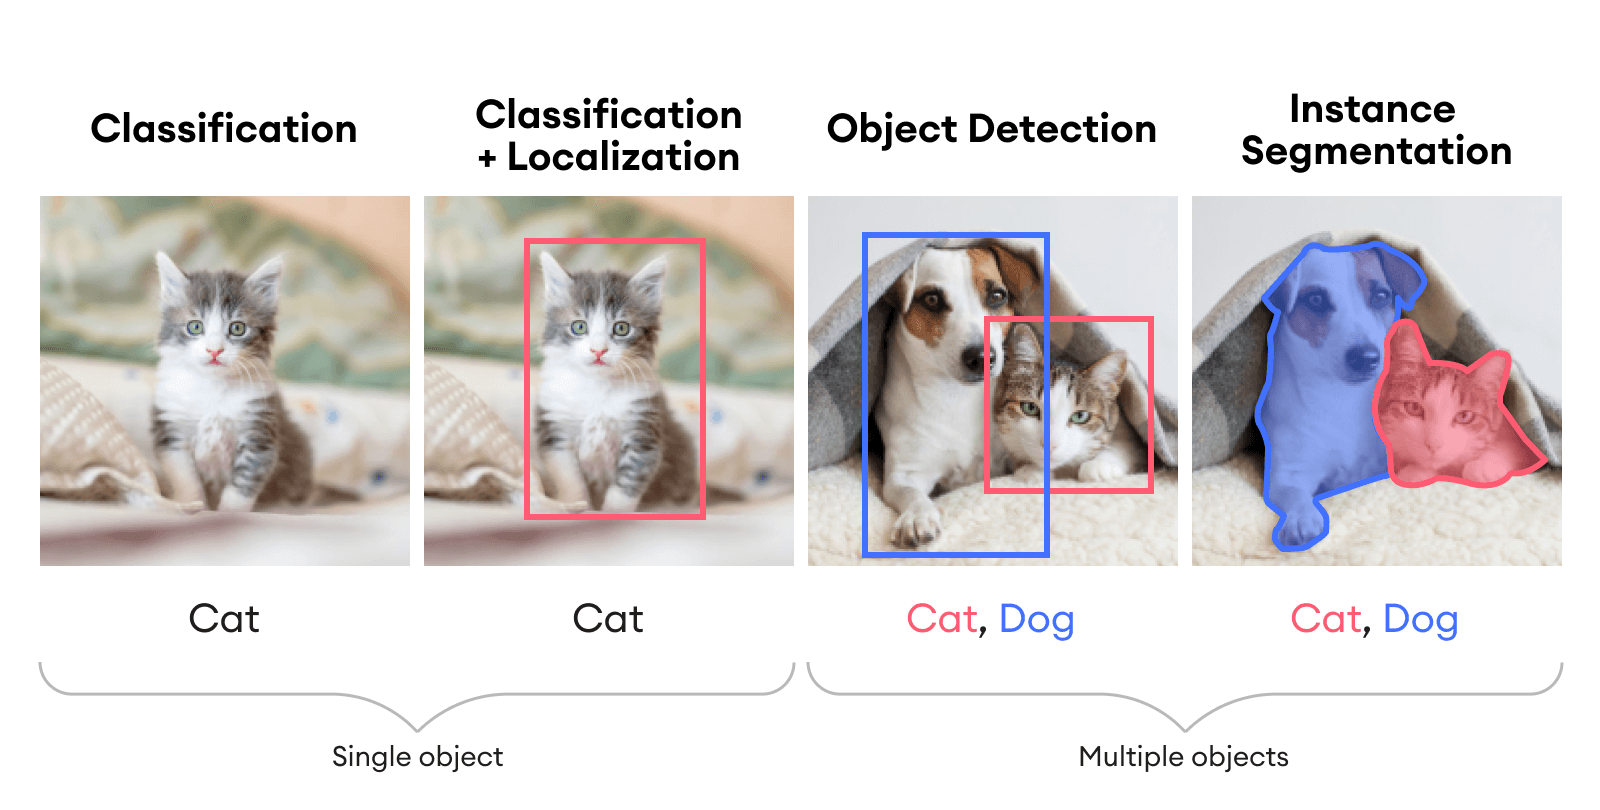
\includegraphics[width=\textwidth]{fig_object_recognition_tasks.png}
    \caption{Object recognition tasks.}
    \label{fig:object_recognition_tasks}
\end{figure}

\subsection{Image classification}
Image classification is a task that assigns a single class label to an image. So, an image classification algorithm takes as input an image with one or more objects and returns a class label. For example, given an image depicting an animal, an image classification model would return one of the labels 'cat', 'dog, 'horse', etc. In the example of Fig. \ref{fig:object_recognition_tasks}, the model returns the class label 'cat'. We do not know the location of the cat in the image. It's important to notice that this task only recognizes a single object in an image, i.e. typically the main object portrayed in the image. 

\subsection{Object localization}
With object localization, we are able to identify the main subject and its location in an image. For this task a model is trained that classifies an image and localizes the main object in that image by generating a bounding box surrounding that object. A bounding box is typically represented by two points: the top-left and bottom-right coordinates of the box. There is only one class label per image as the result of classification. As a consequence, object localization only recognizes objects of the same class. \acrfull{wsol} is an object localization task that only requires image-level labels to learn a model that can localize objects.

\subsection{Object detection}
Object detection is the task of identifying and localizing all objects of interest in an image by assigning a bounding box and class label to each detected object. Hence, an object detection model takes as input an image with one or more objects and returns a set of bounding boxes and corresponding class labels.

\subsection{Instance segmentation}
Instance segmentation detects all instances of a class and demarcates separate instances of any class in an image. It creates a segment map for each instance of class. Consider an image with a cats and a dogas in Fig. \ref{fig:object_recognition_tasks}, instance segmentation enables you to locate bounding boxes of each dog and cat, plot segmentation maps for each dog and cat, and count how many dogs and cats are in the image.

A related task is semantic segmentation. This is a technique to associate a class label with each pixel of a digital image. Essentially, semantic segmentation doesn't classify real-world objects and can't make the distinction between objects.

\section{Artificial neural networks}
State-of-the-art object detection methods are implemented using a \acrfull{ann}. Here, we introduce the basic concepts and terminology of neural networks as we will use those terms further in this document. 

\subsection{Inspiration}
\subsection{Computational model for a neuron}
\subsection{A network of neurons}
\subsection{Hidden layers}

\section{Convolutional neural networks}
\subsection{What is a CNN?}
\subsection{How does it work?}
\subsection{The layers in a CNN}

\section{Supervised learning}
State-of-the-art object detection models are implemented using deep neural networks that are trained using supervised machine learning. Supervised learning for object detection requires that each object in an image must be assigned a class label and a bounding box that localizes the object in the image. This human labeling is a costly and error-prone task. Object localization only deals with recognition of a single object class in an image and can be seen as a simplified object detection task. The goal of the object localization task is to cover the full extent of an object in a digital image.

%(supervised learning, labels, ground-truth, learning)

\section{Weakly supervised object localization}
Human labeling of images with bounding boxes is a costly and error-prone task. Object localization only deals with recognition of a single object class in an image and can be seen as a simplified object detection task. 

\acrshort{wsol} is an object localization task that trains a model by only using image-level labels. Hence the term weakly: Training requires image class labels but no localization bounding boxes. Because costly human labeling of object locations is not required, \acrshort{wsol} research has gained significant momentum \cite{zhou2016cvpr, selvaraju2017grad, chattopadhay2018grad, wang2021minmaxcam, wang2020score, choe2020evaluating}.

The baseline \acrshort{wsol} method is \acrfull{cam} \cite{zhou2016cvpr}. This method trains a model for the classification task and uses learned features that are activated on the most discriminative parts of an object to localize an object of a specific class. This focus on the most discriminative parts is a limitation of the \acrshort{cam} method, as it doesn't cover the complete object. New \acrshort{wsol} research \cite{selvaraju2017grad, chattopadhay2018grad, wang2021minmaxcam, wang2020score, choe2020evaluating} focuses on overcoming the limitations of the baseline \acrshort{cam} method. As the CAM-family of methods represents a main body of research for \acrlong{wsol}, we will use a specific list of CAM methods in this project. The relevant methods will be discussed in chapter \ref{ch:related_work} and \ref{ch:methodology}. 

\section{WSOL and explainability}
%(similarities and differences between wsol and explainability)

The goal of the object localization task is to cover the full extent of an object in a digital image.

Certain CAM-related techniques are mainly used for explainability, i.e. they are used to visually explain why a model predicts a certain class label for an image. Some of these methods indicate the ability to detect multiple object of the same class in an image and show promising results in qualitative experiment results \cite{wang2020score}.

Many \acrshort{cam} papers report performance improvements over the baseline \acrshort{cam} method. Choe \textit{et al.} \cite{choe2020evaluating} criticize that \acrshort{cam} methods lack a unified definition of the \acrshort{wsol} task and proposes a new localization evaluation protocol. A problem is that \acrshort{wsol} has not been tested for localization of multiple object instances of the same class and current \acrshort{wsol} evaluation metrics are not sufficient to measure multiple instance localization. Given that multiple-instance localization hasn't been tested, it is interesting to evaluate it. 

The research question for us is whether we can use CAM-methods to evaluate and improve localization of multiple instances of the same class within images for the \acrshort{wsol} task.

Therefore, we propose an evaluation protocol for localization of multiple-instances of the same class by enhancing existing evaluation metrics \cite{choe2020evaluating} to measure multiple-instance localization performance. We will call this method \acrfull{mwsol}. We then benchmark existing CAM methods for multiple instance localization. Finally, we investigate improvements for the \acrshort{mwsol} task using an iterative bounding box extraction method. Bounding boxes of objects localized in previous iterations, are used to mask their location in images. These masked images are then used to find the location of objects missed during previous iterations.

\section{Looking ahead}
In chapter 2, we discuss the \acrshort{wsol} research that we base our work on: More specifically the family of \acrshort{cam} methods and evaluation methods that we 'll use to benchmark multiple-instance localization. We'll briefly point to \acrshort{wsol} work that is  non-\acrshort{cam} related. 

The methodology used for evaluating \acrlong{mwsol} is explained in detail in chapter 3. We describe the neural networks chosen for implementing the object localization models, the datasets for training the models and the \acrshort{cam} methods for object localization. We define enhancements of existing \acrshort{wsol} metrics required to evaluate localization of multiple instances and we explain an improvement strategy for localizing multiple instances.

We describe the results of our experiments in chapter 4. For each method the computational complexity, localization performance are provided. Chapter 5 provides a detailed discussion of the experiment results. Our conclusions on \acrshort{mwsol} are explained in chapter 6.